\documentclass[ignorenonframetext,]{beamer}
\setbeamertemplate{caption}[numbered]
\setbeamertemplate{caption label separator}{: }
\setbeamercolor{caption name}{fg=normal text.fg}
\beamertemplatenavigationsymbolsempty
\usepackage{lmodern}
\usepackage{amssymb,amsmath}
\usepackage{ifxetex,ifluatex}
\usepackage{fixltx2e} % provides \textsubscript
\ifnum 0\ifxetex 1\fi\ifluatex 1\fi=0 % if pdftex
  \usepackage[T1]{fontenc}
  \usepackage[utf8]{inputenc}
\else % if luatex or xelatex
  \ifxetex
    \usepackage{mathspec}
  \else
    \usepackage{fontspec}
  \fi
  \defaultfontfeatures{Ligatures=TeX,Scale=MatchLowercase}
\fi
\usetheme[]{Antibes}
\usecolortheme{dolphin}
\usefonttheme{structurebold}
% use upquote if available, for straight quotes in verbatim environments
\IfFileExists{upquote.sty}{\usepackage{upquote}}{}
% use microtype if available
\IfFileExists{microtype.sty}{%
\usepackage{microtype}
\UseMicrotypeSet[protrusion]{basicmath} % disable protrusion for tt fonts
}{}
\newif\ifbibliography
\hypersetup{
            pdftitle={Random projection to dimention reduction of large scale data},
            pdfauthor={Siamak Dehbod Supervisor Dr.~Adel Mohammadpour Advisor Dr.~Hadi Zare},
            pdfborder={0 0 0},
            breaklinks=true}
\urlstyle{same}  % don't use monospace font for urls
\usepackage{graphicx,grffile}
\makeatletter
\def\maxwidth{\ifdim\Gin@nat@width>\linewidth\linewidth\else\Gin@nat@width\fi}
\def\maxheight{\ifdim\Gin@nat@height>\textheight0.8\textheight\else\Gin@nat@height\fi}
\makeatother
% Scale images if necessary, so that they will not overflow the page
% margins by default, and it is still possible to overwrite the defaults
% using explicit options in \includegraphics[width, height, ...]{}
\setkeys{Gin}{width=\maxwidth,height=\maxheight,keepaspectratio}

% Prevent slide breaks in the middle of a paragraph:
\widowpenalties 1 10000
\raggedbottom

\AtBeginPart{
  \let\insertpartnumber\relax
  \let\partname\relax
  \frame{\partpage}
}
\AtBeginSection{
  \ifbibliography
  \else
    \let\insertsectionnumber\relax
    \let\sectionname\relax
    \frame{\sectionpage}
  \fi
}
\AtBeginSubsection{
  \let\insertsubsectionnumber\relax
  \let\subsectionname\relax
  \frame{\subsectionpage}
}

\setlength{\parindent}{0pt}
\setlength{\parskip}{6pt plus 2pt minus 1pt}
\setlength{\emergencystretch}{3em}  % prevent overfull lines
\providecommand{\tightlist}{%
  \setlength{\itemsep}{0pt}\setlength{\parskip}{0pt}}
\setcounter{secnumdepth}{0}

\title{Random projection to dimention reduction of large scale data}
\author{Siamak Dehbod \newline \newline Supervisor Dr.~Adel Mohammadpour
\newline Advisor Dr.~Hadi Zare}
\institute{Amirkabir University of Technology}
\date{January 20, 2019}

\begin{document}
\frame{\titlepage}

\begin{frame}
\tableofcontents[hideallsubsections]
\end{frame}

\section{Indroduction}\label{indroduction}

\subsection{Masive Data}\label{masive-data}

\begin{frame}{Large Scale Data}

\begin{itemize}
\tightlist
\item
  more dimensions than records (D \textgreater{} n)
\item
  unable to compute \(A^T A\) and using \emph{PCA}
\item
  online/stream calculation
\item
  unable to store whole data
\item
  covariance is not finite
\end{itemize}

\end{frame}

\begin{frame}{Big Data}

\begin{itemize}
\tightlist
\item
  Volume
\item
  Velocity
\item
  Variety
\end{itemize}

\end{frame}

\begin{frame}{Heavy tail data}

\begin{itemize}
\item
  Common in real data like market data, rare events are more probable
  than normal distribution
\item
  Random variable \(X\) with right side heavy-tail distribution:
\end{itemize}

\[ P(X > x) \sim cx^{-\alpha}, x \rightarrow \infty\]

\end{frame}

\subsection{Dimention Reduction}\label{dimention-reduction}

\begin{frame}{Random Coordinate Sampling}

Pros:

\begin{itemize}
\tightlist
\item
  Simplicity \(O(nk)\)
\item
  Flexability for estimating various summary statistics
\end{itemize}

Cons:

\begin{itemize}
\tightlist
\item
  Not accurate for losing rare events
\item
  Not suitable for sparse data
\end{itemize}

\end{frame}

\begin{frame}{Principal components analysis}

\begin{figure}
\centering
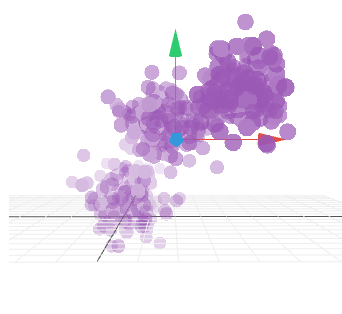
\includegraphics{pics/09-1.png}
\caption{}
\end{figure}

\end{frame}

\begin{frame}{Principal components analysis}

\begin{figure}
\centering
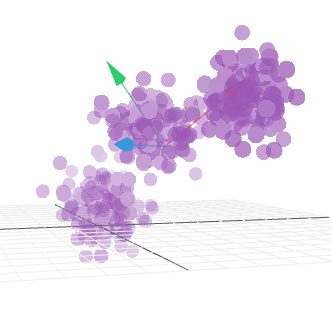
\includegraphics{pics/09-2.png}
\caption{}
\end{figure}

\end{frame}

\subsection{Clustring}\label{clustring}

\begin{frame}{Clustering}

\begin{figure}
\centering
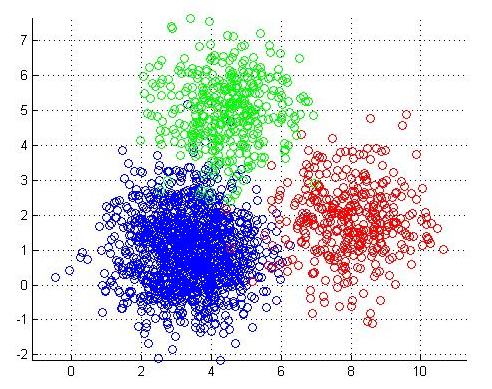
\includegraphics{pics/03.png}
\caption{Clustering}
\end{figure}

\end{frame}

\begin{frame}{k-means}

Non-hierarchical clustering method

minimize within-cluster sum of squares

\[\underset{\mathbf{S}} {\operatorname{arg\,min}}  \sum_{i=1}^{k} \sum_{\mathbf x \in S_i} \left\| \mathbf x - \boldsymbol\mu_i \right\|^2 = \underset{\mathbf{S}} {\operatorname{arg\,min}}  \sum_{i=1}^{k} |S_i| \operatorname{Var} S_i \]

\end{frame}

\begin{frame}{Adjusted Rand Index}

\[\frac{a+b}{a+b+c+d}\]

\end{frame}

\begin{frame}{Adjusted Rand Index}

\begin{table}[h]
\centering
\begin{tabular}{l|llll|l}
Class \textbackslash Cluster & $v_1$    & $v_2$  & $\ldots$ & $v_C$  & Sums      \\ \hline
$u_1$                        & $n_{11}$ & $n_{12}$ & $\ldots$ & $n_{1C}$ & $n_{1.}$     \\
$u_2$                        & $n_{21}$ & $n_{22}$ & $\ldots$ & $n_{2C}$ & $n_{2.}$     \\
$\vdots$                     & $\vdots$ & $\vdots$ & $\ddots$ & $\vdots$ & $\vdots$     \\
$u_R$                        & $n_{R1}$ & $n_{R2}$ & $\ldots$ & $n_{RC}$ & $n_{R.}$     \\ \hline
Sums                         & $n_{.1}$ & $n_{.2}$ & $\ldots$ & $n_{.C}$ & $n_{..} = n$
\end{tabular}
\label{tab:1iY}
\end{table}

\end{frame}

\begin{frame}{Adjusted Rand Index}

\begin{align}
\frac{ 
    \sum_{i,j} \binom{n_{ij}}{2}
    -
    \left[ \sum_i \binom{n_{i.}}{2} \sum_j \binom{n_{.j}}{2} \right] / \binom{n}{2}
 }{
    \frac{1}{2} 
    \left[ 
        \sum_i 
        \binom{n_{i.}}{2}
        +
        \sum_j
        \binom{n_{.j}}{2}
    \right]
    -
    \left[ \sum_i \binom{n_{i.}}{2} \sum_j \binom{n_{.j}}{2} \right] / \binom{n}{2}
}
\label{eq:1ix}
\end{align}

\end{frame}

\begin{frame}{\(C_e\)}

\[ C_e = 100 (\mathrm{ARI}_d - \mathrm{ARI}_p  ) \] \[ (d<p) \]

\end{frame}

\subsection{Applications}\label{applications}

\begin{frame}{Distances}

\begin{align}
a=u_1^T u_2 = \sum_{i=1}^{D} u_{1,i} u_{2,i} \\
d_{(\alpha)} = \sum_{i=1}^{D} \mathopen| u_1 - u_2 \mathclose|^\alpha 
\label{eq:1hP}
\end{align}

\end{frame}

\begin{frame}{Distances}

\[ A^T A : O(n^2D)\]

\[ O(n^2 \hat{f}) \]

\end{frame}

\begin{frame}{Database Query Optimization}

joins and execution plan

\end{frame}

\begin{frame}{Sub-linear Nearest Neighbor Searching}

\[ O(nD) \rightarrow O(nk) \]
\[ (\alpha > 1) l_\alpha \rightarrow O(n^\gamma) (\gamma < 1) \]

\end{frame}

\section{Stable Random Projection}\label{stable-random-projection}

\subsection{Stable Distribution}\label{stable-distribution}

\begin{frame}{Stable Distribution}

\begin{figure}
\centering
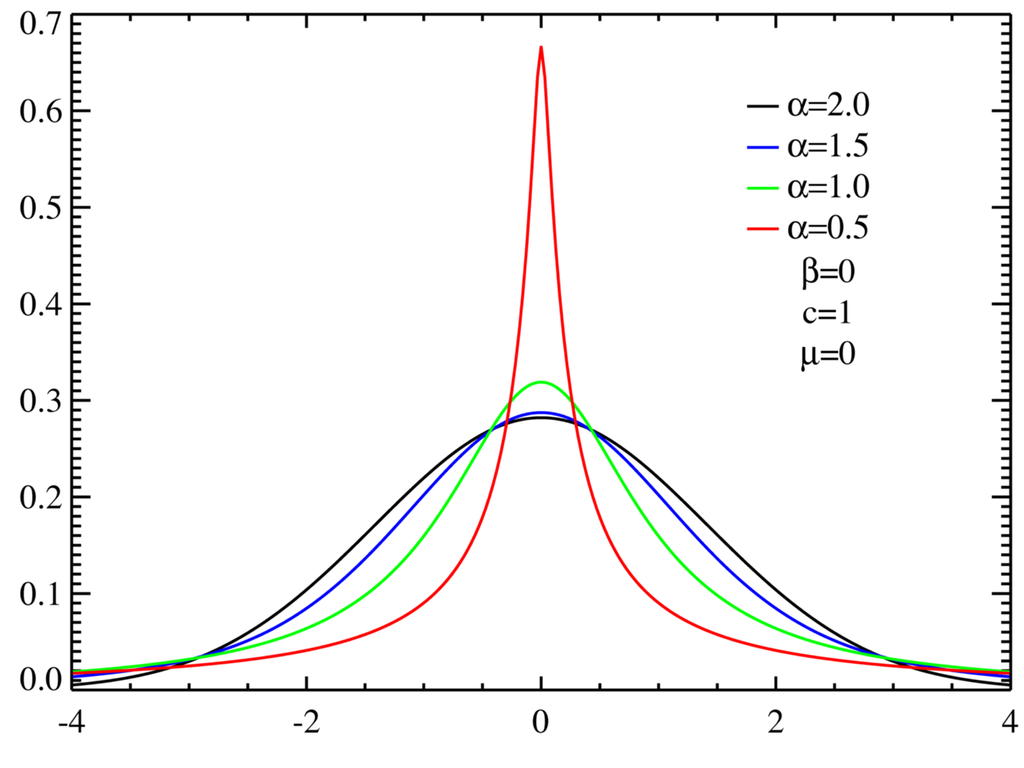
\includegraphics{pics/04.png}
\caption{Stable distribution}
\end{figure}

\end{frame}

\begin{frame}{Stable Distribution}

\[ X_1 + X_2 + \cdots + X_n =^d c_n X + d_n \] Gaussian/normal:
\[ f(x) = (2\pi)^{1/2} \exp (-x^2/2)\] Cauchy:

\[ f(x) = 1/(\pi(1+x^2)) \]

\end{frame}

\begin{frame}{Stable Normal N(0,1)}

\begin{figure}
\centering
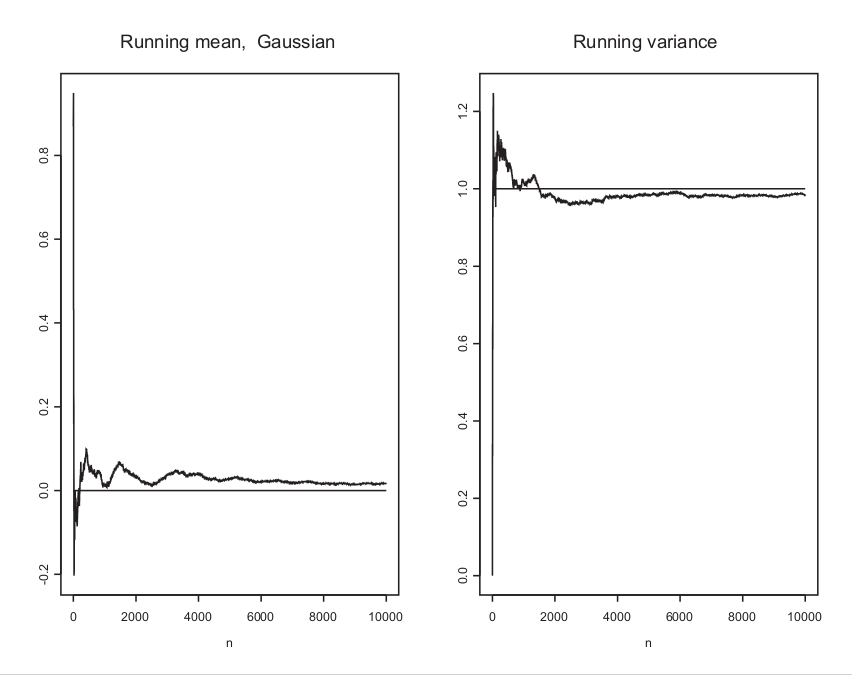
\includegraphics{pics/05.png}
\caption{Normal \(\alpha = 2\)}
\end{figure}

\end{frame}

\begin{frame}{Stable \(\alpha = 1.5\)}

\begin{figure}
\centering
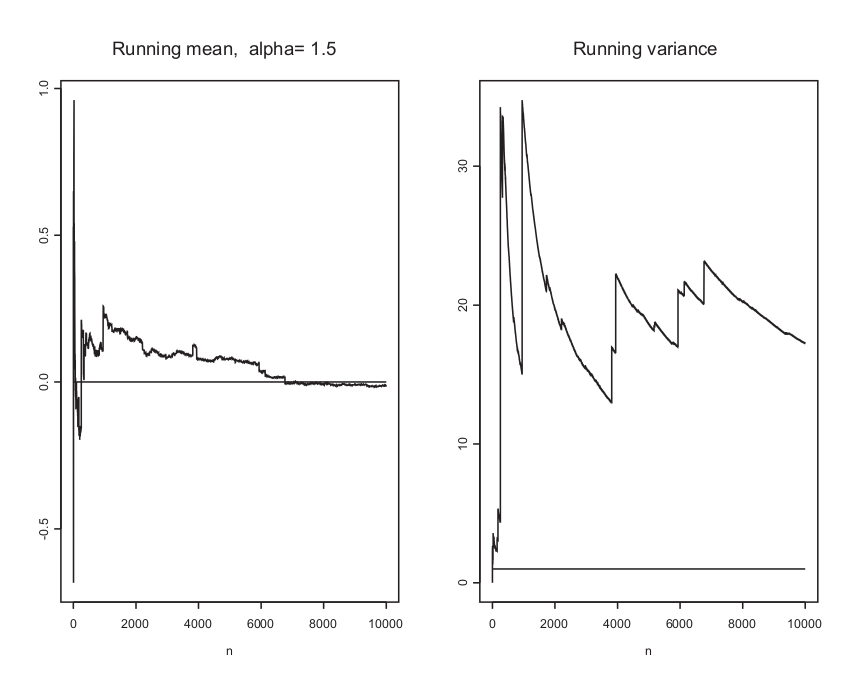
\includegraphics{pics/06.png}
\caption{\(\alpha = 1.5\)}
\end{figure}

\end{frame}

\begin{frame}{Stable \(\alpha = 0.75\)}

\begin{figure}
\centering
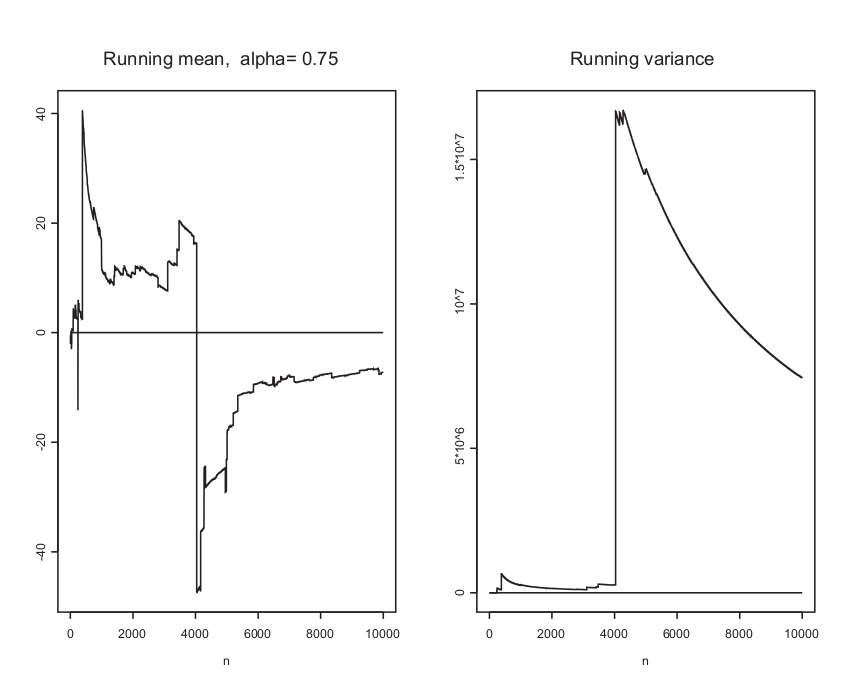
\includegraphics{pics/07.png}
\caption{\(\alpha = 0.75\)}
\end{figure}

\end{frame}

\subsection{Stable Random Projection}\label{stable-random-projection-1}

\begin{frame}{Stable Random Projection}

\begin{figure}
\centering
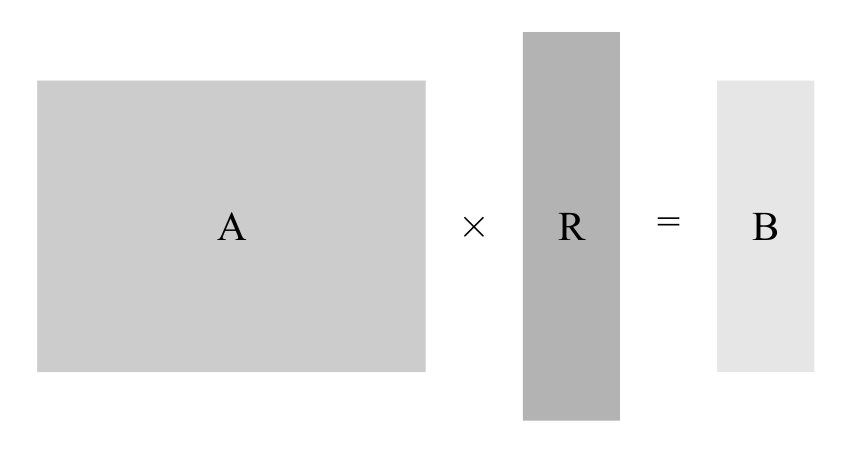
\includegraphics{pics/10.png}
\caption{}
\end{figure}

\end{frame}

\begin{frame}{Stable Random Projection}

Johnson-Lindenstrauss Lemma:

\[ k = O \left ( \frac{\log n}{\epsilon^2 } \right ) \]
\[ l_2: 1 \pm \epsilon\]

\end{frame}

\begin{frame}{Statistical estimation problem}

\begin{align}
v_{1,j} \sim S \bigg( \alpha, \sum_{i=1}^D |u_{1,i}|^\alpha \bigg), \;\;
v_{2,j} \sim S \bigg( \alpha, \sum_{i=1}^D |u_{2,i}|^\alpha \bigg),\\
x_j = v_{1,j} - v_{2,j} \sim S \bigg( \alpha, d_{(\alpha)} = 
\sum_{i=1}^D | u_{1,i} - u_{2,i} |^\alpha \bigg).
\end{align}

\end{frame}

\begin{frame}{Couchy Random Projection}

\[d = \sum_{i=1}^D | u_{1,i} - u_{2,i} | \]

\end{frame}

\begin{frame}{Very Sparse Random Projection}

\[\left\{ -1, 0, 1 \right\}\]

\[\left\{ \frac{1}{2s}, 1 - \frac{1}{s}, \frac{1}{2s} \right\}\]

\[ O(Dk) \rightarrow O(Dk/s) \]

\end{frame}

\begin{frame}{\(l_\alpha\) Random Projection}

\[d_{(\alpha)} = \sum_{i=1}^D \left| u_{1,i} - u_{2,i} \right|^{\alpha}\]

\end{frame}

\section{Data \& Implementation}\label{data-implementation}

\begin{frame}{Data summary}

\begin{center}


\begin{tabular}{l|r|r|r}
\hline
Dataset & $n$ & $D$ & $N_{class}$\\
\hline
Thyroid & 215 & 5 & 3\\
\hline
Iris & 150 & 4 & 3\\
\hline
Diabetes & 145 & 3 & 3\\
\hline
Swiss Banknotes & 200 & 6 & 2\\
\hline
Seeds & 210 & 7 & 3\\
\hline
Mice Protein Expression & 1080 & 77 & 8\\
\hline
Crabs & 200 & 6 & 2\\
\hline
\end{tabular}

\end{center}

\end{frame}

\section{Results}\label{results}

\begin{frame}{\(C_e\)}

\[ C_e = 100 (\mathrm{ARI}_d - \mathrm{ARI}_p  ) \] \[ (d<p) \]

\end{frame}

\subsection{\texorpdfstring{Normal
\(\alpha = 2, d = 2\)}{Normal \textbackslash{}alpha = 2, d = 2}}\label{normal-alpha-2-d-2}

\begin{frame}{Tabel \(\alpha = 2, d = 2\)}

\begin{center}


\begin{tabular}{l|r|r|r}
\hline
Dataset & ${ARI}_p$ & ${ARI}_d$ & $C_e$\\
\hline
Thyroid & 0.58 & 0.40 & -18\\
\hline
Iris & 0.62 & 0.47 & -15\\
\hline
Diabetes & 0.38 & 0.36 & -2\\
\hline
Swiss Banknotes & 0.85 & 0.39 & -46\\
\hline
Seeds & 0.77 & 0.45 & -33\\
\hline
Mice Protein Expression & 0.13 & 0.07 & -7\\
\hline
Crabs & 0.05 & 0.04 & 0\\
\hline
\end{tabular}

\end{center}

\end{frame}

\begin{frame}{Histogram 2 peak}

\begin{center}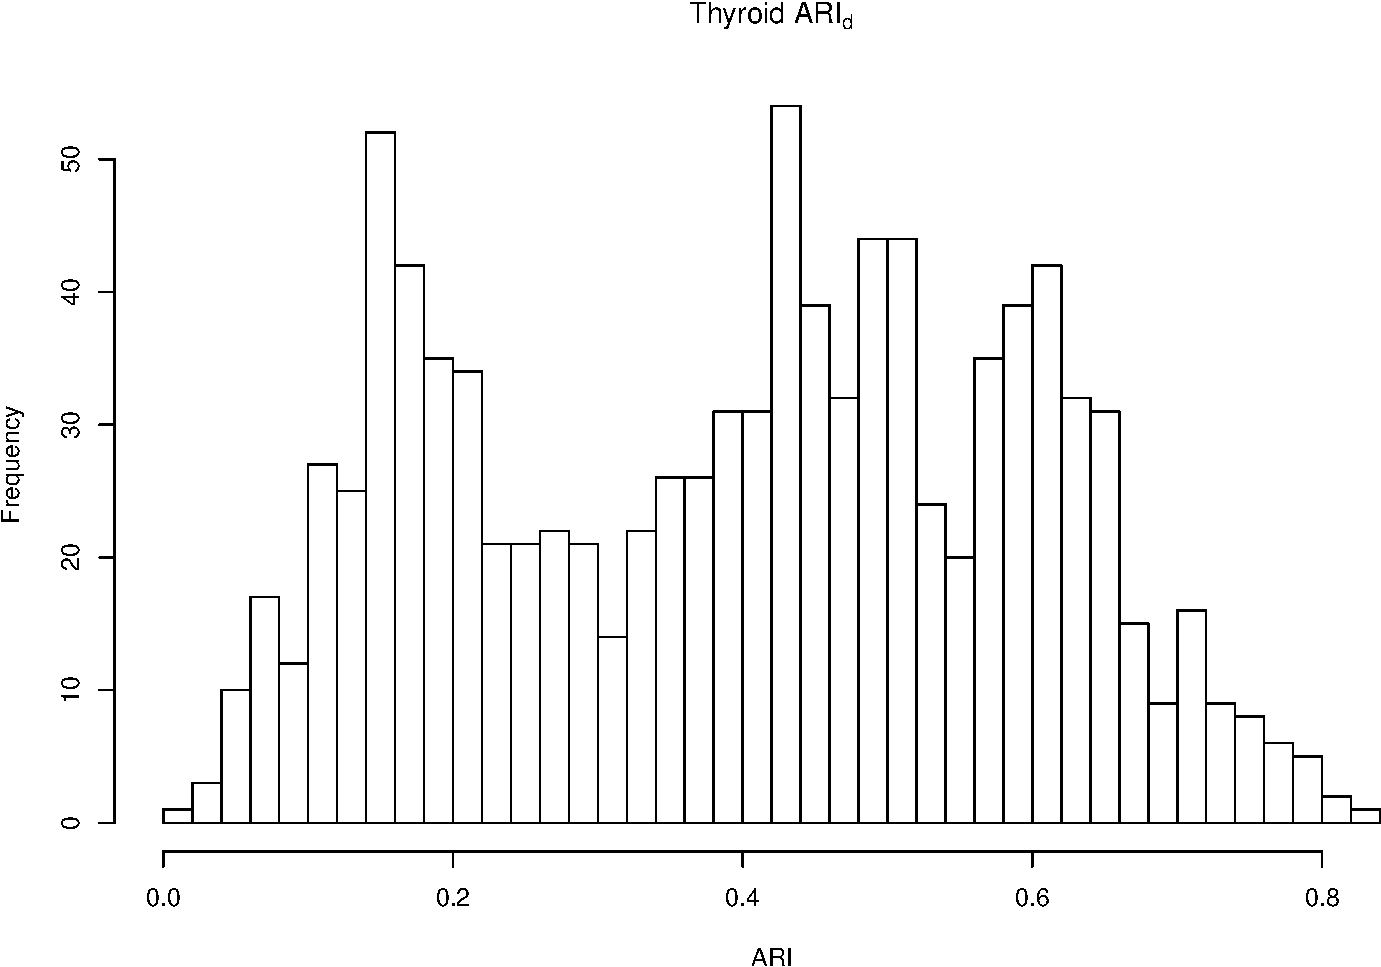
\includegraphics[width=1\linewidth]{Presentation_files/figure-beamer/unnamed-chunk-5-1} \end{center}

\end{frame}

\begin{frame}{Hisogram undefined}

\begin{center}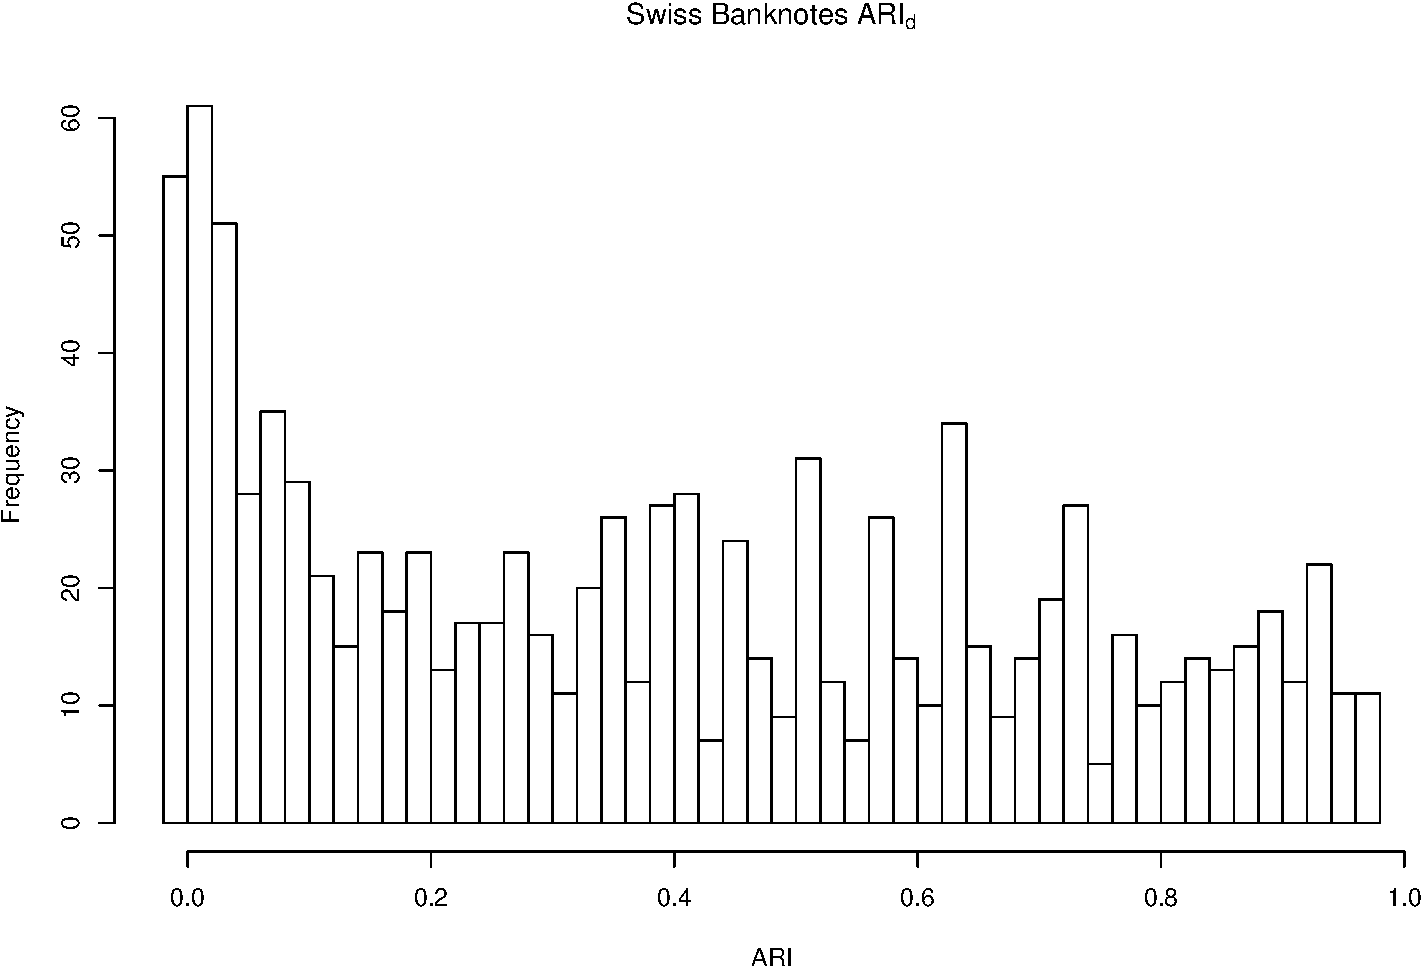
\includegraphics[width=1\linewidth]{Presentation_files/figure-beamer/unnamed-chunk-6-1} \end{center}

\end{frame}

\begin{frame}{Hisogram efficient}

\begin{center}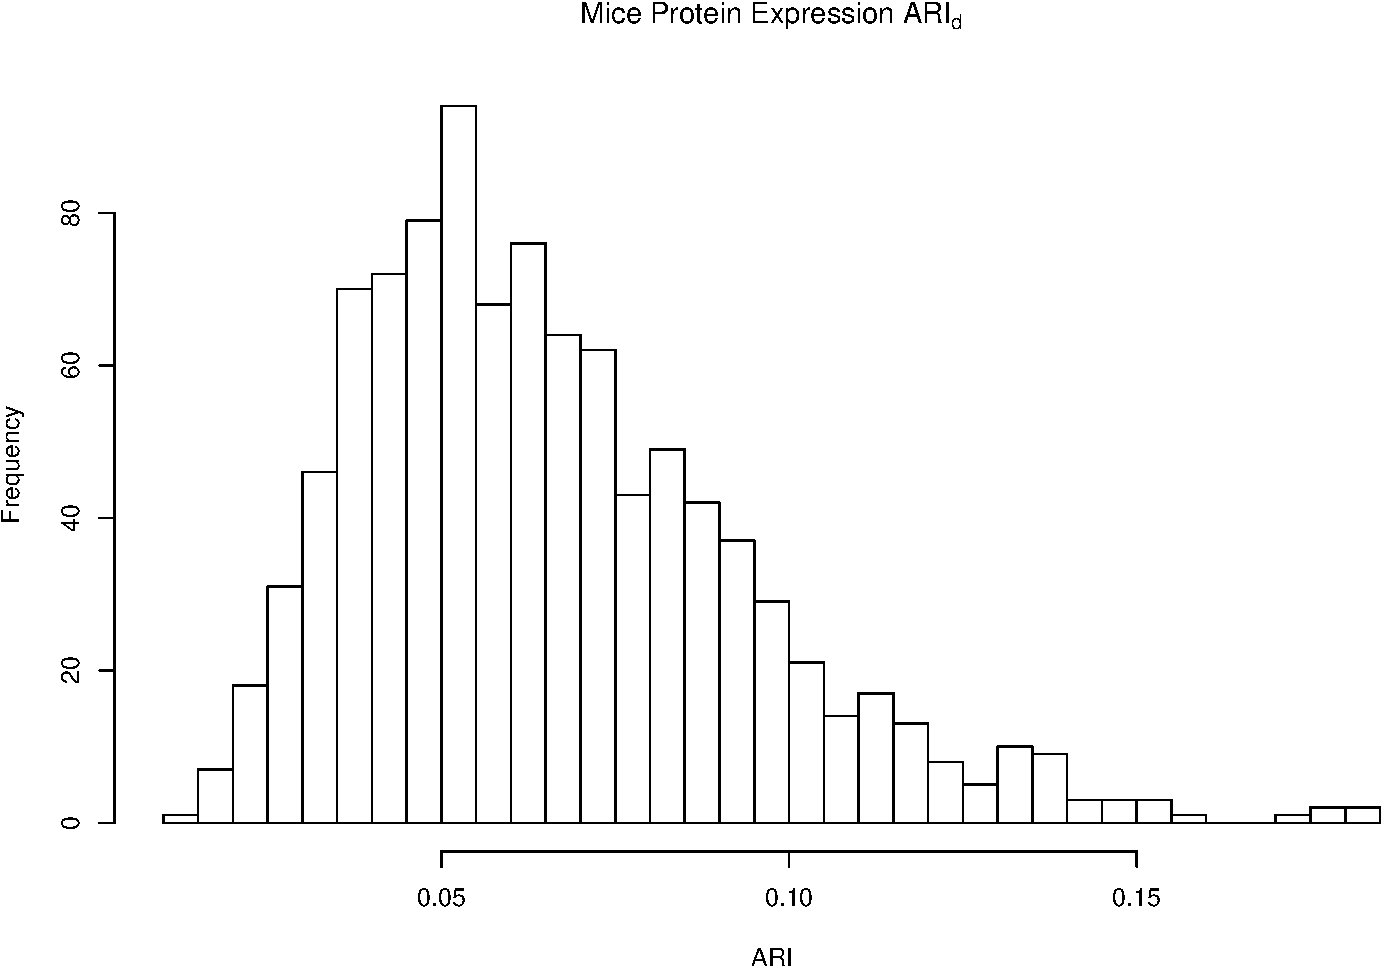
\includegraphics[width=1\linewidth]{Presentation_files/figure-beamer/unnamed-chunk-7-1} \end{center}

\end{frame}

\subsection{\texorpdfstring{Normal
\(\alpha = 2, d = 3\)}{Normal \textbackslash{}alpha = 2, d = 3}}\label{normal-alpha-2-d-3}

\begin{frame}{Tabel \(\alpha = 2, d = 3\)}

\begin{center}


\begin{tabular}{l|r|r|r}
\hline
Dataset & ${ARI}_p$ & ${ARI}_d$ & $C_e$\\
\hline
Thyroid & 0.58 & 0.43 & -15\\
\hline
Iris & 0.62 & 0.54 & -8\\
\hline
Diabetes & 0.38 & 0.38 & 0\\
\hline
Swiss Banknotes & 0.85 & 0.47 & -37\\
\hline
Seeds & 0.77 & 0.53 & -24\\
\hline
Mice Protein Expression & 0.13 & 0.08 & -5\\
\hline
Crabs & 0.05 & 0.05 & 0\\
\hline
\end{tabular}

\end{center}

\end{frame}

\subsection{\texorpdfstring{Cauchy
\(\alpha = 1, d = 2\)}{Cauchy \textbackslash{}alpha = 1, d = 2}}\label{cauchy-alpha-1-d-2}

\begin{frame}{Tabel \(\alpha = 1, d = 2\)}

\begin{center}


\begin{tabular}{l|r|r|r}
\hline
Dataset & ${ARI}_p$ & ${ARI}_d$ & $C_e$\\
\hline
Thyroid & 0.58 & 0.36 & -23\\
\hline
Iris & 0.62 & 0.51 & -11\\
\hline
Diabetes & 0.38 & 0.33 & -5\\
\hline
Swiss Banknotes & 0.85 & 0.40 & -44\\
\hline
Seeds & 0.77 & 0.45 & -32\\
\hline
Mice Protein Expression & 0.13 & 0.06 & -7\\
\hline
Crabs & 0.05 & 0.05 & 0\\
\hline
\end{tabular}

\end{center}

\end{frame}

\subsection{\texorpdfstring{Cauchy
\(\alpha = 1, d = 3\)}{Cauchy \textbackslash{}alpha = 1, d = 3}}\label{cauchy-alpha-1-d-3}

\begin{frame}{Tabel \(\alpha = 1, d = 3\)}

\begin{center}


\begin{tabular}{l|r|r|r}
\hline
Dataset & ${ARI}_p$ & ${ARI}_d$ & $C_e$\\
\hline
Thyroid & 0.58 & 0.37 & -22\\
\hline
Iris & 0.62 & 0.54 & -8\\
\hline
Diabetes & 0.38 & 0.35 & -3\\
\hline
Swiss Banknotes & 0.85 & 0.43 & -41\\
\hline
Seeds & 0.77 & 0.47 & -30\\
\hline
Mice Protein Expression & 0.13 & 0.07 & -7\\
\hline
Crabs & 0.05 & 0.05 & 0\\
\hline
\end{tabular}

\end{center}

\end{frame}

\subsection{\texorpdfstring{Sparse
\(s = 2, d = 2\)}{Sparse s = 2, d = 2}}\label{sparse-s-2-d-2}

\begin{frame}{Tabel \(s = 2, d = 2\)}

\begin{center}


\begin{tabular}{l|r|r|r}
\hline
Dataset & ${ARI}_p$ & ${ARI}_d$ & $C_e$\\
\hline
Thyroid & 0.58 & 0.40 & -18\\
\hline
Iris & 0.62 & 0.49 & -13\\
\hline
Diabetes & 0.38 & 0.35 & -3\\
\hline
Swiss Banknotes & 0.85 & 0.40 & -44\\
\hline
Seeds & 0.77 & 0.45 & -33\\
\hline
Mice Protein Expression & 0.13 & 0.06 & -7\\
\hline
Crabs & 0.05 & 0.05 & 0\\
\hline
\end{tabular}

\end{center}

\end{frame}

\subsection{\texorpdfstring{Sparse
\(s = 2, d = 3\)}{Sparse s = 2, d = 3}}\label{sparse-s-2-d-3}

\begin{frame}{Tabel \(s = 2, d = 3\)}

\begin{center}


\begin{tabular}{l|r|r|r}
\hline
Dataset & ${ARI}_p$ & ${ARI}_d$ & $C_e$\\
\hline
Thyroid & 0.58 & 0.44 & -14\\
\hline
Iris & 0.62 & 0.54 & -8\\
\hline
Diabetes & 0.38 & 0.37 & -1\\
\hline
Swiss Banknotes & 0.85 & 0.49 & -36\\
\hline
Seeds & 0.77 & 0.53 & -24\\
\hline
Mice Protein Expression & 0.13 & 0.08 & -5\\
\hline
Crabs & 0.05 & 0.05 & 0\\
\hline
\end{tabular}

\end{center}

\end{frame}

\subsection{\texorpdfstring{\(C_e\) versus \(\alpha\) for
\(d = 2\)}{C\_e versus \textbackslash{}alpha for d = 2}}\label{c_e-versus-alpha-for-d-2}

\begin{frame}{Normal is better}

\begin{center}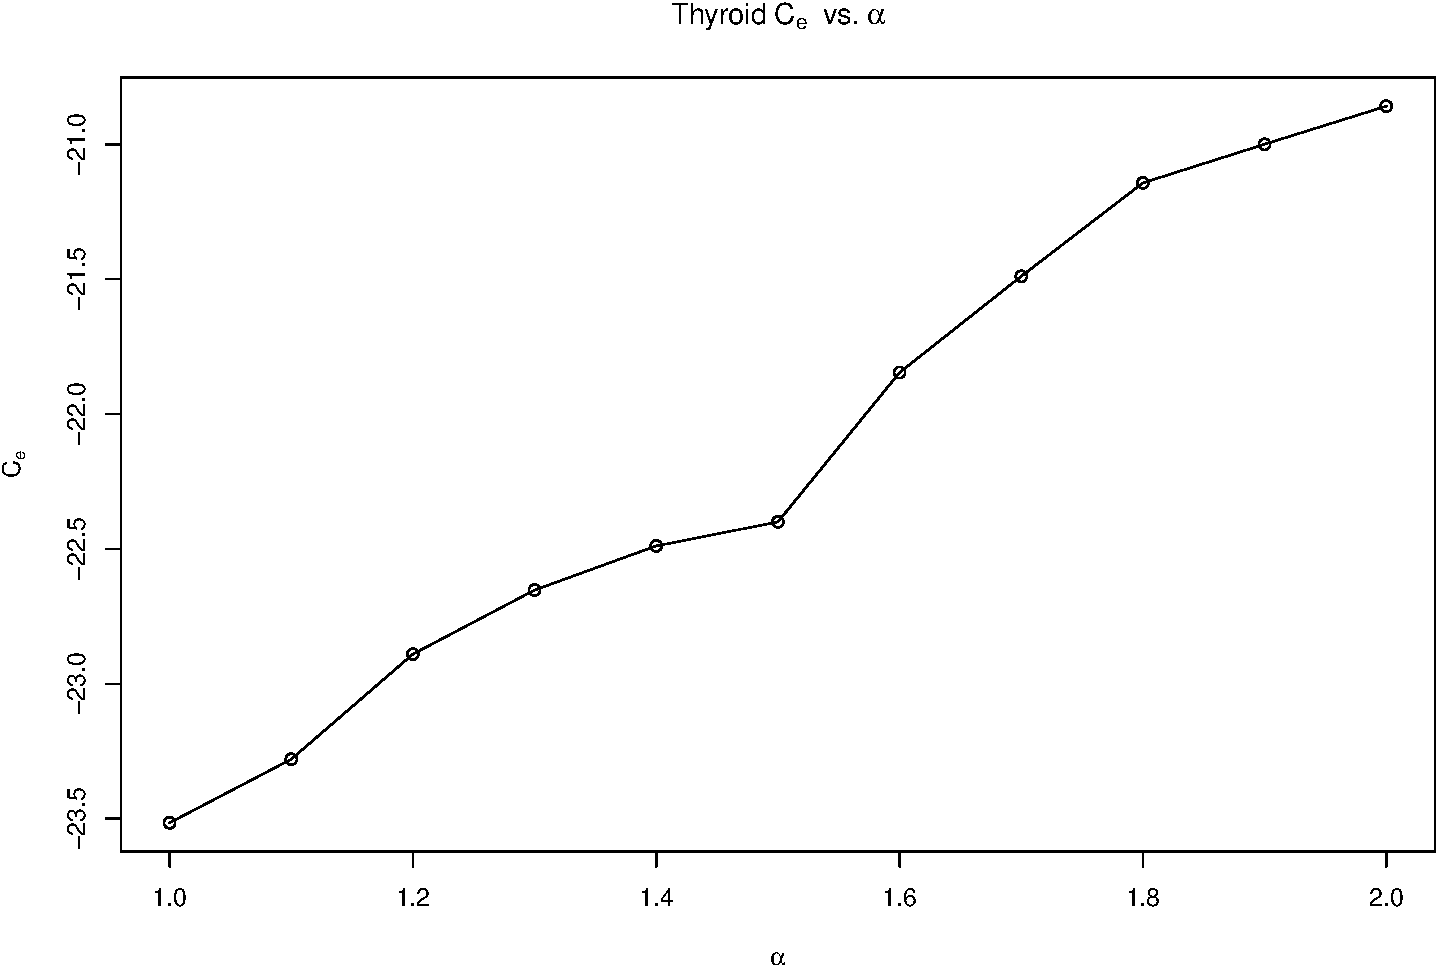
\includegraphics[width=1\linewidth]{Presentation_files/figure-beamer/unnamed-chunk-19-1} \end{center}

\end{frame}

\begin{frame}{Cauchy is better}

\begin{center}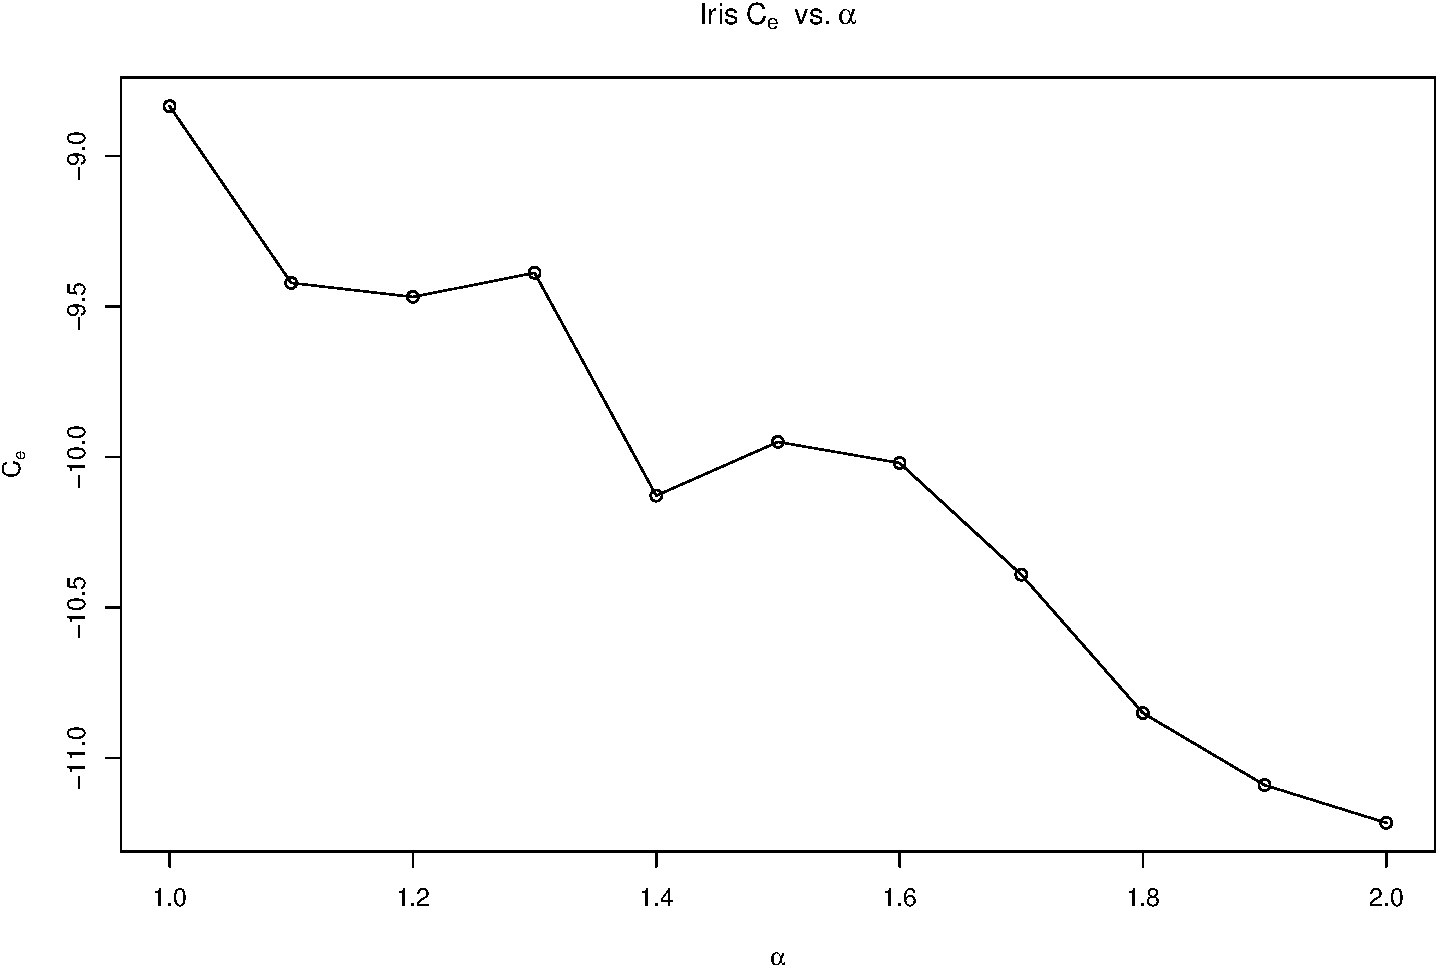
\includegraphics[width=1\linewidth]{Presentation_files/figure-beamer/unnamed-chunk-20-1} \end{center}

\end{frame}

\begin{frame}{\(0<\alpha<1\) is better}

\begin{center}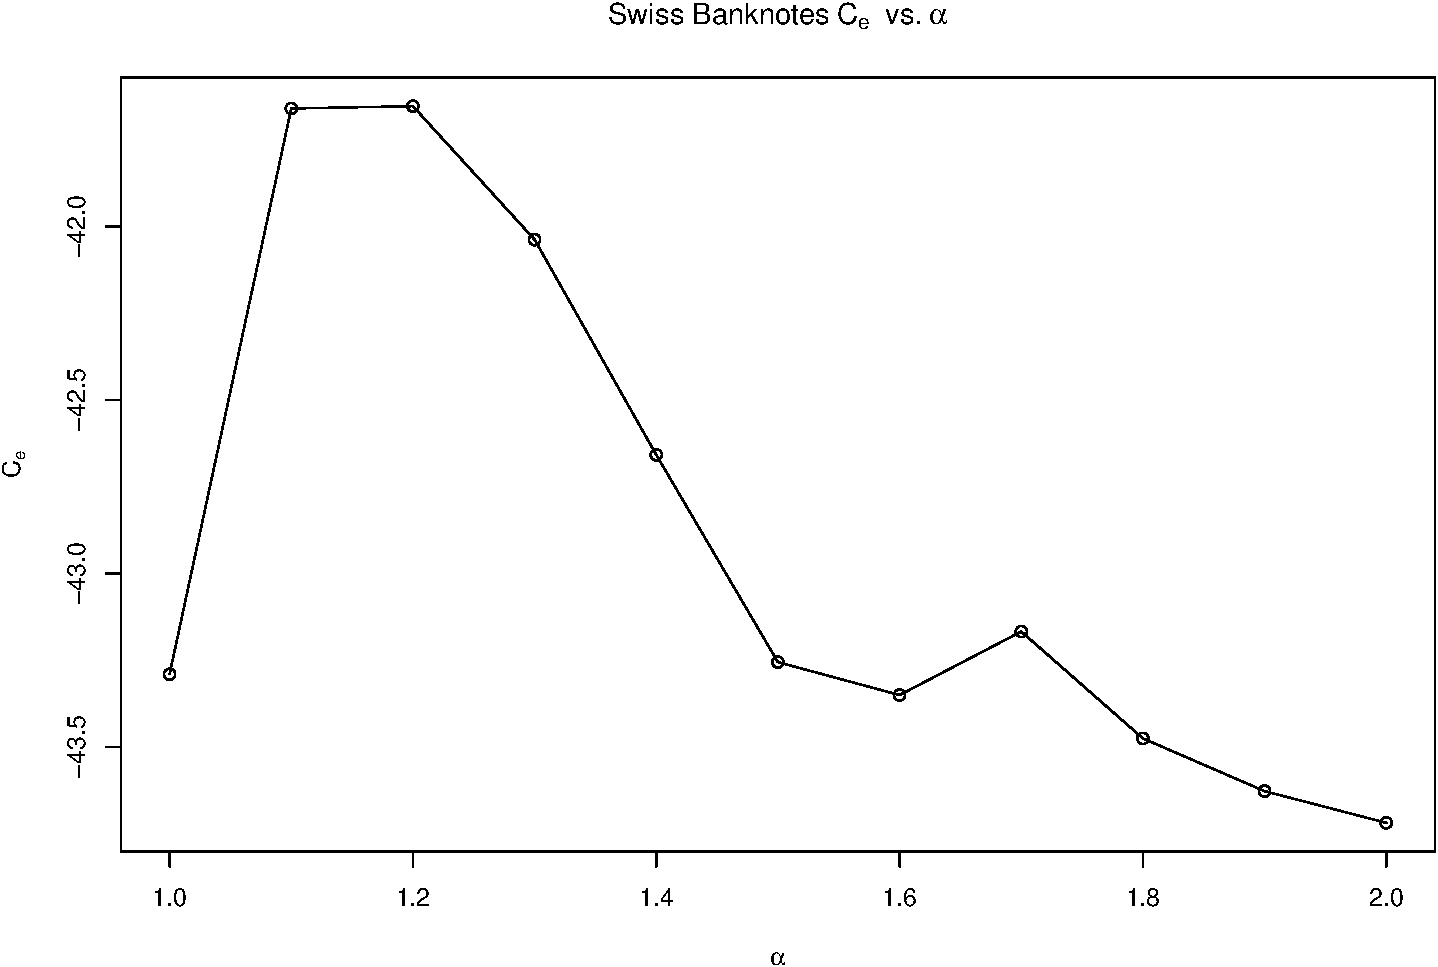
\includegraphics[width=1\linewidth]{Presentation_files/figure-beamer/unnamed-chunk-21-1} \end{center}

\end{frame}

\subsection{\texorpdfstring{\(C_e\) versus \(\alpha\) for
\(d = 3\)}{C\_e versus \textbackslash{}alpha for d = 3}}\label{c_e-versus-alpha-for-d-3}

\begin{frame}{Normal is better}

\begin{center}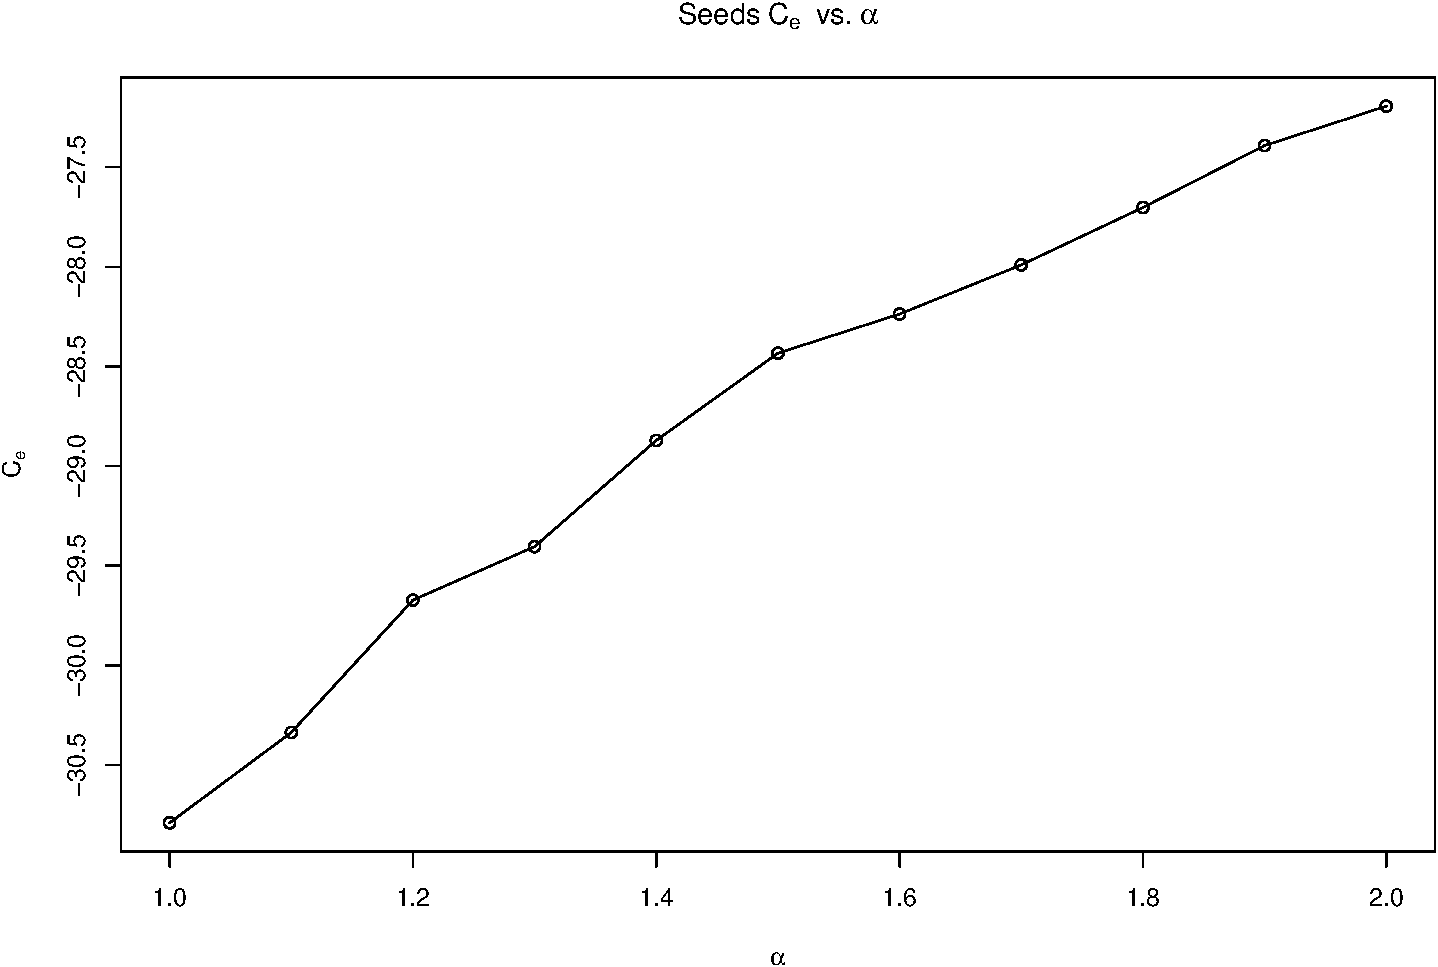
\includegraphics[width=1\linewidth]{Presentation_files/figure-beamer/unnamed-chunk-23-1} \end{center}

\end{frame}

\begin{frame}{Cauchy is better}

\begin{center}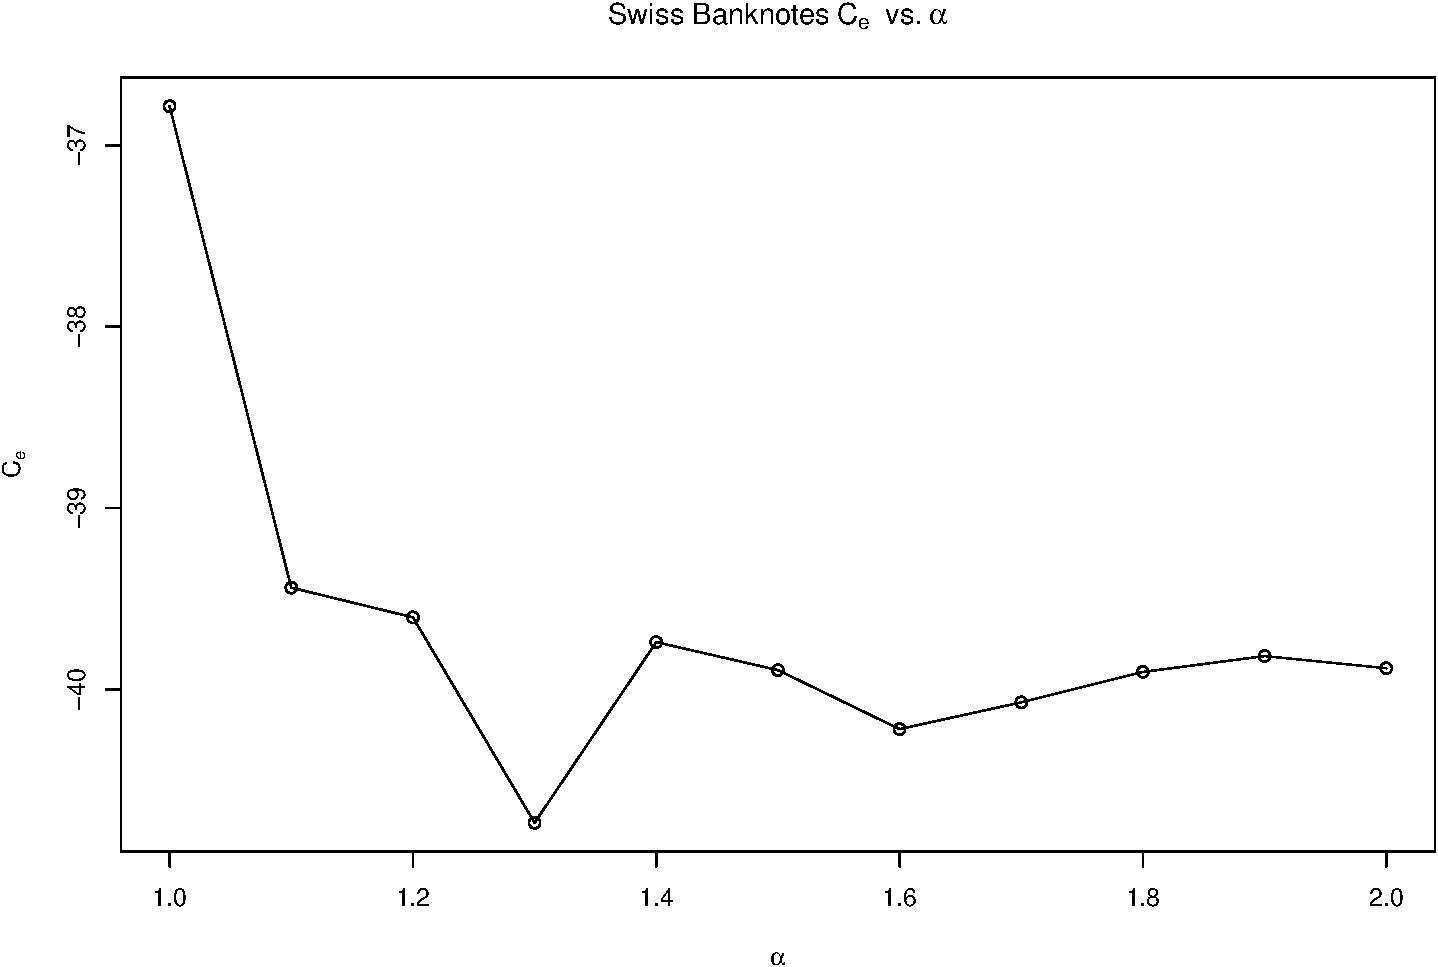
\includegraphics[width=1\linewidth]{Presentation_files/figure-beamer/unnamed-chunk-24-1} \end{center}

\end{frame}

\begin{frame}{\(0<\alpha<1\) is better}

\begin{center}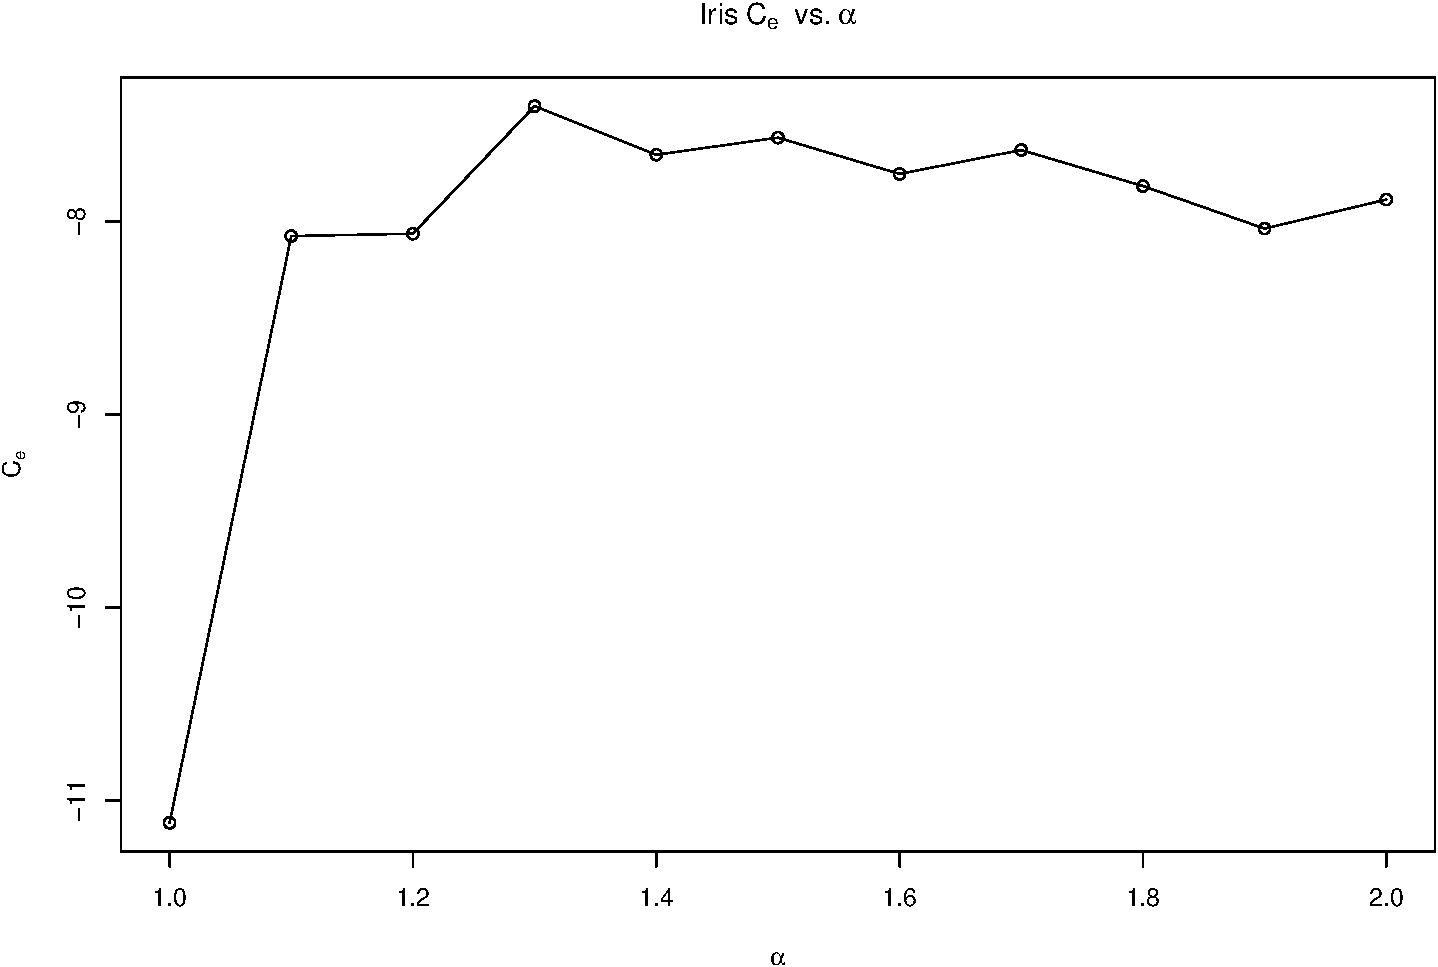
\includegraphics[width=1\linewidth]{Presentation_files/figure-beamer/unnamed-chunk-25-1} \end{center}

\end{frame}

\subsection{\texorpdfstring{\(C_e\) versus \(s\) in Sparse for
\(d = 2\)}{C\_e versus s in Sparse for d = 2}}\label{c_e-versus-s-in-sparse-for-d-2}

\begin{frame}{MPE}

\begin{center}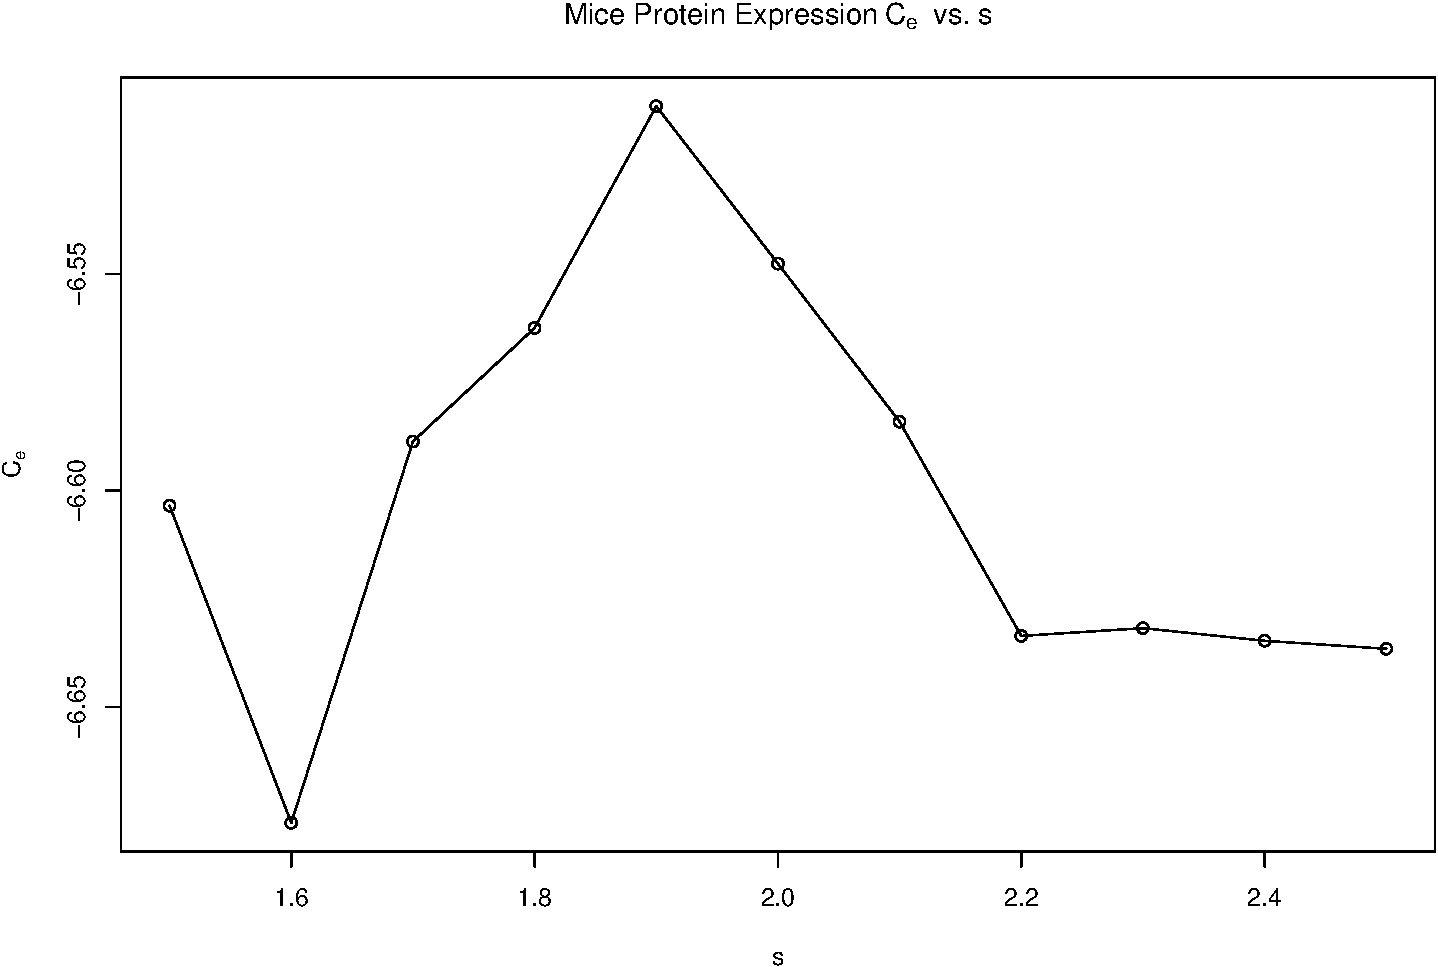
\includegraphics[width=1\linewidth]{Presentation_files/figure-beamer/unnamed-chunk-27-1} \end{center}

\end{frame}

\subsection{\texorpdfstring{\(C_e\) versus \(s\) in Sparse for
\(d = 3\)}{C\_e versus s in Sparse for d = 3}}\label{c_e-versus-s-in-sparse-for-d-3}

\begin{frame}{Seeds}

\begin{center}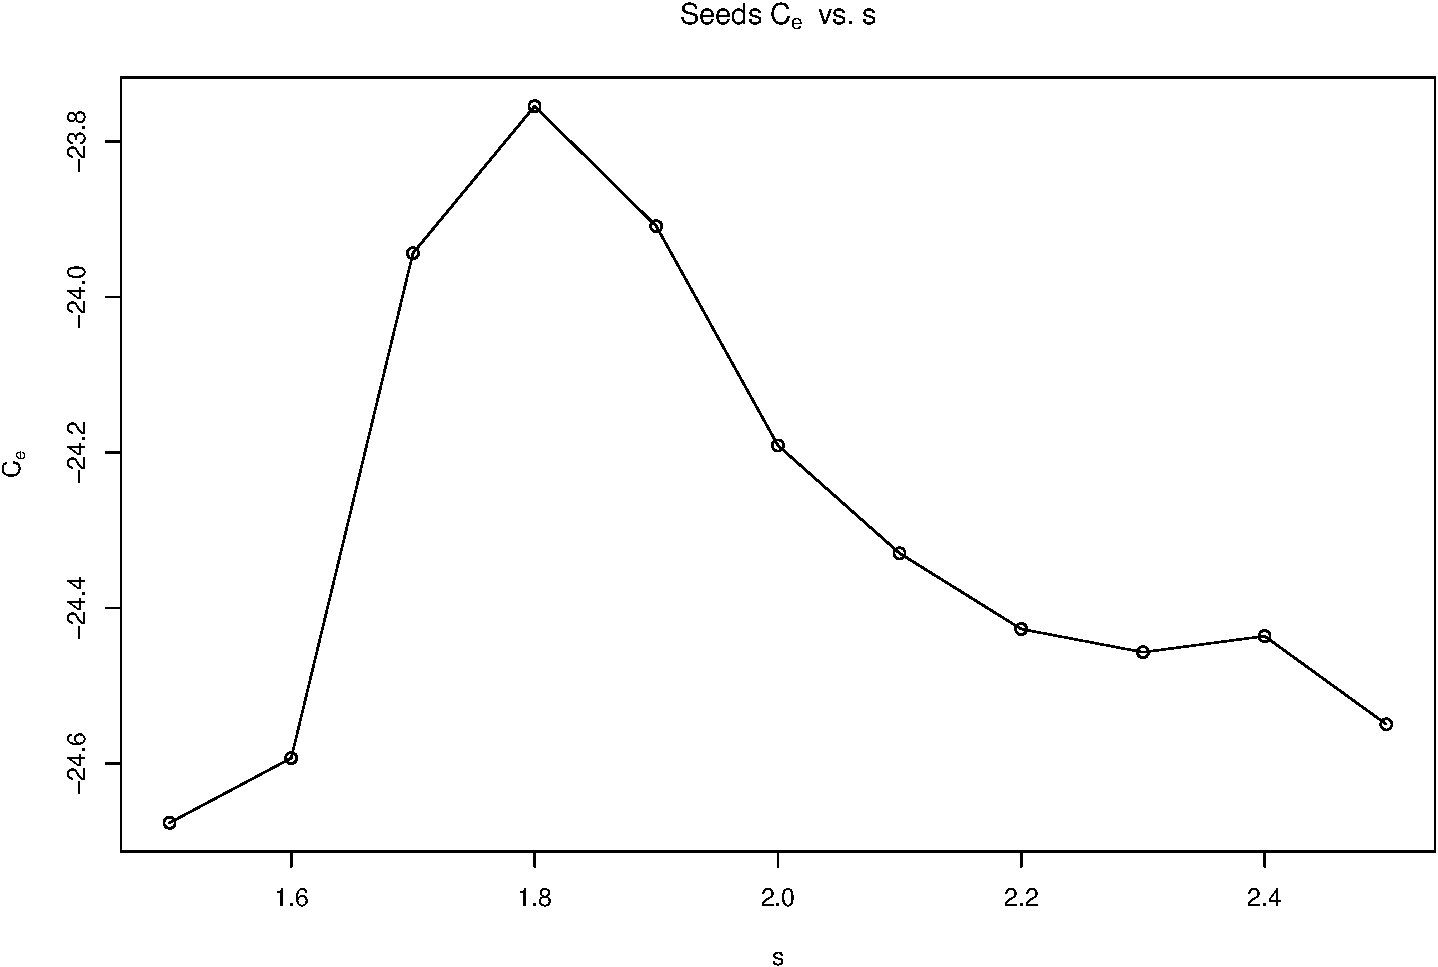
\includegraphics[width=1\linewidth]{Presentation_files/figure-beamer/unnamed-chunk-29-1} \end{center}

\end{frame}

\subsection{\texorpdfstring{Comparision
\(d = 2\)}{Comparision d = 2}}\label{comparision-d-2}

\begin{frame}{Comparision \(d = 2\)}

\begin{figure}
\centering
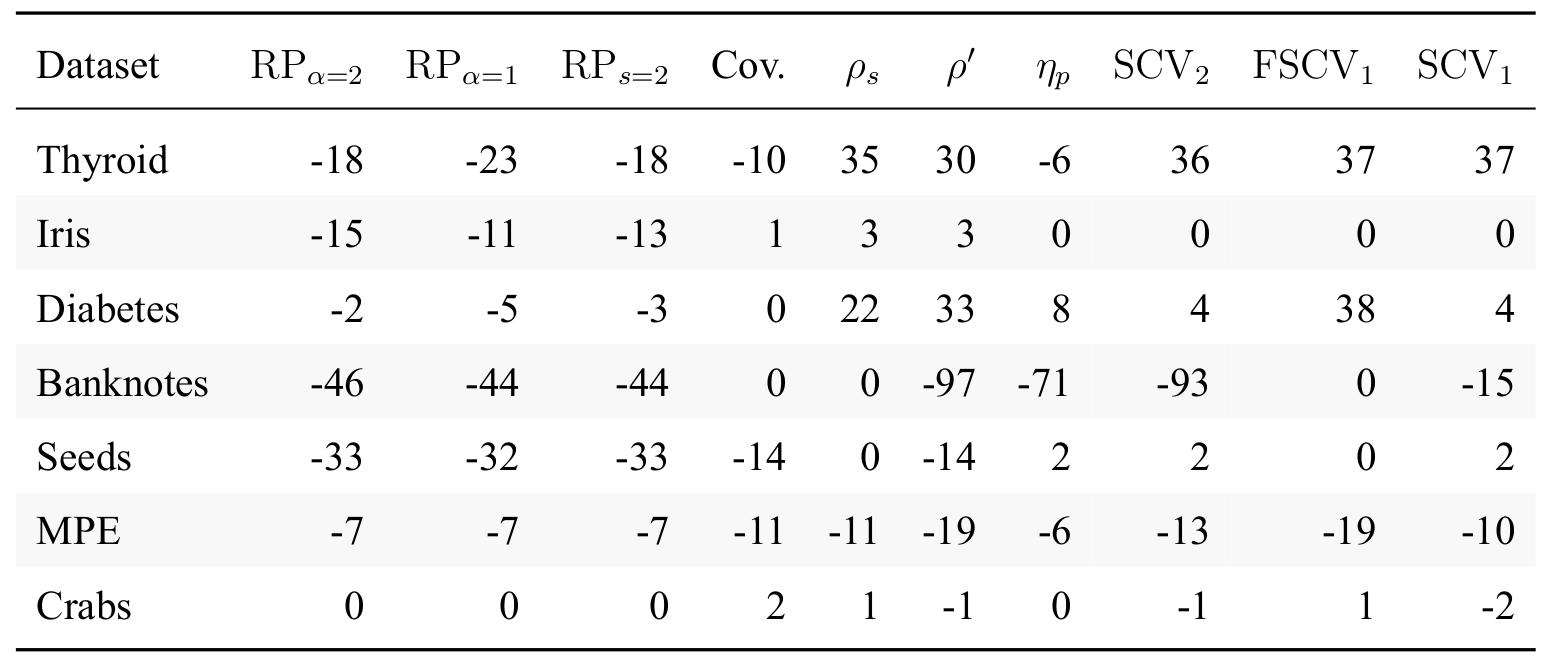
\includegraphics{pics/01.png}
\caption{d = 2}
\end{figure}

\end{frame}

\subsection{\texorpdfstring{Comparision
\(d = 3\)}{Comparision d = 3}}\label{comparision-d-3}

\begin{frame}{Comparision \(d = 3\)}

\begin{figure}
\centering
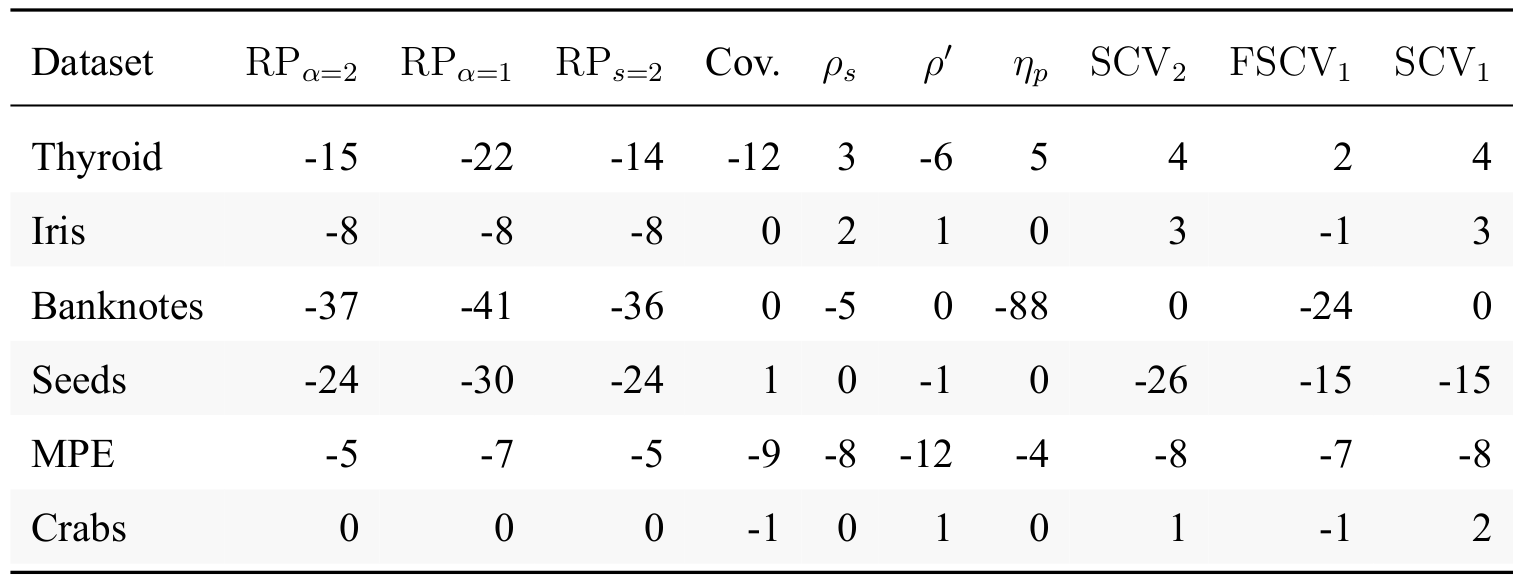
\includegraphics{pics/02.png}
\caption{d = 3}
\end{figure}

\end{frame}

\subsection{???}\label{section}

\begin{frame}{Similarity measures}

\begin{figure}
\centering
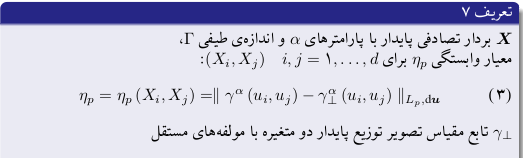
\includegraphics{pics/08-1.png}
\caption{}
\end{figure}

\end{frame}

\begin{frame}{Similarity measures}

\begin{figure}
\centering
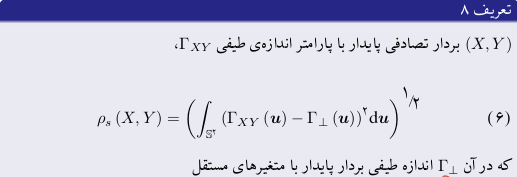
\includegraphics{pics/08-2.png}
\caption{}
\end{figure}

\end{frame}

\begin{frame}{Similarity measures}

\begin{figure}
\centering

\includegraphics{pics/08-3.png}
\caption{}
\end{figure}

\end{frame}

\begin{frame}{Similarity measures}

\begin{figure}
\centering
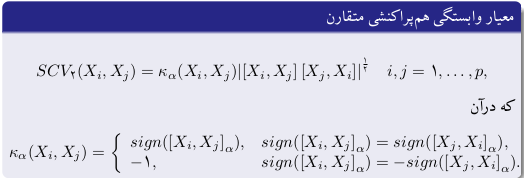
\includegraphics{pics/08-4.png}
\caption{}
\end{figure}

\end{frame}

\end{document}
